\documentclass[../main.tex]{subfiles}

\begin{document}
\section{CHIPs Architecture}
The CHIPS architecture is an amalgamation of chiplets connected through an interposer. This structure is known as two and a half Dimensions (2.5D), and this structure is the foundation of the CHIPS architecture. The technology that allows chiplets to communication through an interposer is (AIB) advanced interface bus\cite{AIBWhitePaper}. This bus severs as the physical layer in the protocol stack. All chiplets use AXI as the next layer in the protocol stack. AXI is the protocol that makes up the buck of the SOC for the CHIPS architecture.

\subsection{2.5D Structure}
All chiplets share a standard interface in the CHIPS architecture, AIB interface. This interface allows chiplet to chiplet communication through an interposer, and figure \ref{fig:AIBInterposer} shows the structure of this interface. Each chiplet's IO consists of an AIB driver. This driver is capable of running at a single data rate (SDR) or double data rate (DDR). SDR is the configuration used in the CHIPS architecture. The AIB drivers work in pairs, one set to transmit and the other set to receive. Figure \ref{fig:AIBInterface} shows a standard configuration of drivers. An AIB channel is a collection of AIB drivers, and figure \ref{fig:AIBChannel} shows one such channel.  For transfer data across this interface, one channel must be a master, and the other must be a slave. The AIB interface makes up the lowest link in the protocol stack. The next physical link in the protocol stack is the AXI interface, and all the chiplets share this interface.    

\begin{figure}
    \centering
    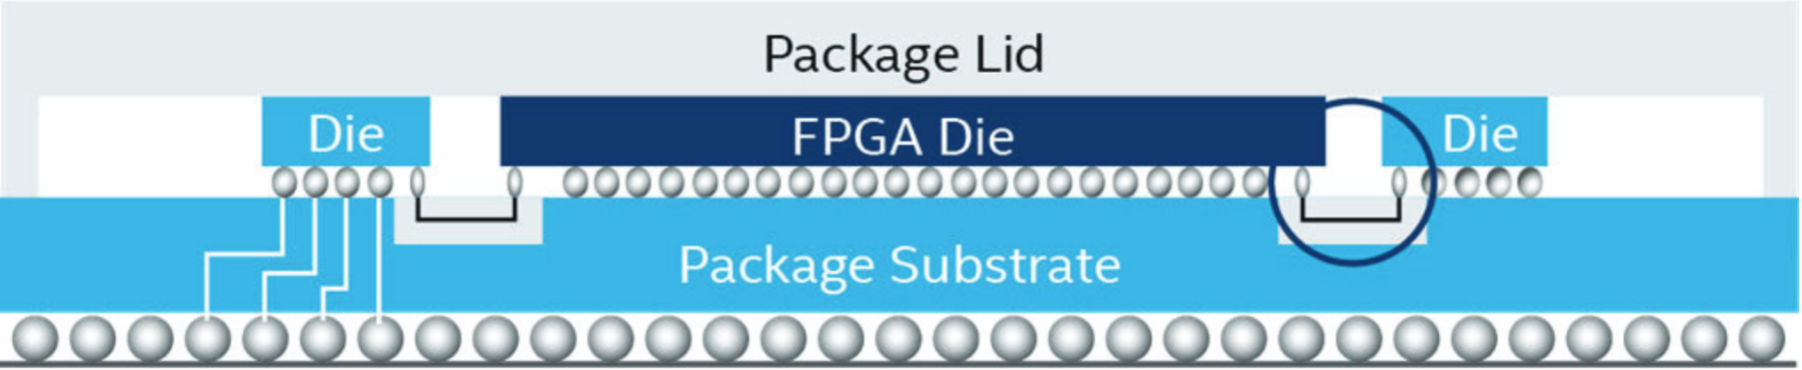
\includegraphics[scale=.25]{pngs/Interposer.png}
    \caption{AIB Interposer Connection\cite{AIBWhitePaper}}
    \label{fig:AIBInterposer}
\end{figure}
\begin{figure}
    \centering
    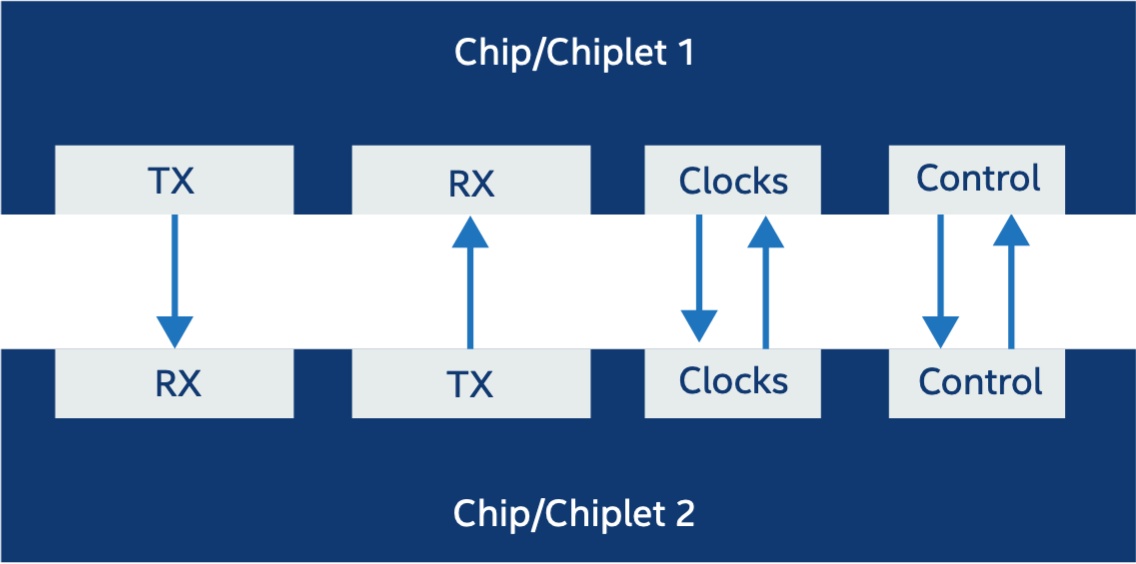
\includegraphics[scale=.4]{pngs/AIB-interface.png}
    \caption{AIB Interface\cite{AIBWhitePaper}}
    \label{fig:AIBInterface}
\end{figure}

\begin{figure}
    \centering
    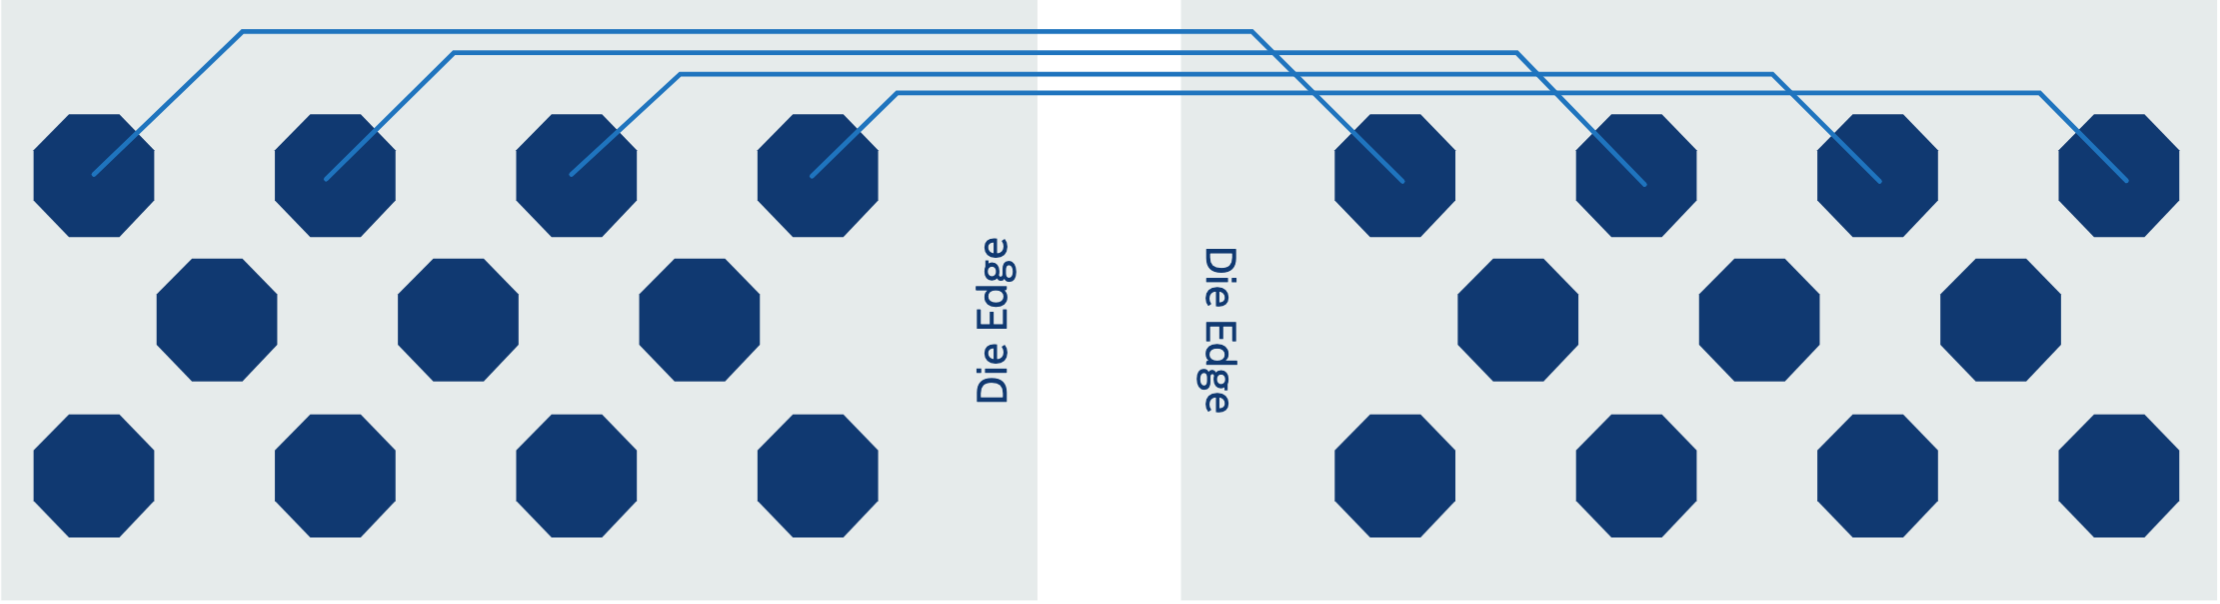
\includegraphics[scale=.2]{pngs/AIB-Channel.png}
    \caption{AIB Channel Connection\cite{AIBWhitePaper}}
    \label{fig:AIBChannel}
\end{figure}

An AIB channel in the CHIPS architecture is made up of 48 drivers. The drivers are broken up into two functions: one is data transfer, and the other is transmitting or receiving 4 sets of differential clocks. The lower 40 drivers are for data, and the upper 8 are for clocks. The configuration of the drivers depends on which side of the AIB interface the driver is on. For master, the data drivers are set to transmit, and the other drivers are set to receive, and the same goes for the clocks. Theses clocks create an async boundary around each chiplet. 

The four clocks are broken up into two groups: master launch and slave launch, and both groups work in the same way. Each group includes two clocks, one is generated, and the other is received. These clock groups are broken up into three parts: the transmitter clock (Tx), the receiver clock (Rx), and the feedback clock (Rx\texttt{\_}Tx). Figures 1, 2, and 3 show these clock configuration. Tx clock transmit data from the sender to the receiver, and the Rx cock receives data from the sender. Final, the forward clock is used to transmit data on the sender's clock edge. Data transfer from master to slave when all three parts are connected.

\subsection{CHIPS SOC}
For phase one, there is no interposer. Therefore, AIB drivers connect through standard routing. AIB drivers stack needs to support both a top-level connection and a lower metal connection.  Because of limited area in phase one, AIB wraps around only one of the Rocket core chips. Therefore, each AIB driver on the Rocker core side has to have a corresponding AIB driver on the crosspoint side.

The CHIPs SOC connects chiplets through a support structure. This structure consists of one on-chip memory bus (MBus), one off-chip memory bus (ExMBus), one control bus (XBus), and five debug buses.  Through the XBus, the Rocket cores gain access to the neural network chiplets. The MBus provides access to the on-chip and off-chip memory controller for all of the chiplets. The ExMBus connects off-chip memory to the off-chip memory controller.  Both of the on-chip buses, XBus and MBus, are AXI based, and the off-chip memory bus, ExMBus, is CIPI based. 

\subsection{Chiplets}
Each chiplet has three bus connections. For controller chiplets, Rocket cores, it has two master AXI ports, XBus and MBus, and one Jtag debug port. For the neural network chiplets, it has one master AXI port, MBus, one slave AXI port, XBus, and one Jtag debug port.

%The controllers chiplets use the Rocket Chip IP\cite{Asanović:EECS-2016-17}. In this layout, there are two different layouts for the Rocket Chip, one was wrapped with AIB and the other was not. The two accelerators chiplets are LSTM and SCNN. Figure ?? shows the layout of the tape-out. Each major Design is hi highlighted. 
\subsubsection{Rocket Core}
The Rocket core had to be modified to work in the CHIPs architecture. In this version of the Rocket core, there is no floating-point hardware, and there is support for the custom instructions extensions. Only one of the custom instruction extensions is used to control access to the XBus. This instruction has two variants, bus read and bus write. These two actions allow the Rocket core to control and debug the neural network chiplets via XBus. See figure ?? for the layout of this version of the Rocket core. Figure ?? shows the layout of the new Rocket chiplet.
\subsubsection{Neural Network Chiplets}
In this architecture, there are two neural network chiplets: LSTM and SCNN. Both chiplets are accessible via Jtag port or XBus port. These chiplets are designed to work at the coarse grain programming level. 

The first chiplet of interest is the long short term chiplet (LSTM). At NCSU, Dr. Summon Dey designed this chiplet for his Ph.D. The following is an overview of his design. His design focuses on developing hardware that can fully utilization memory bandwidth. His design is scalable with the amount of memory bandwidth available. In addition to being scalable, it needed to be sensitive changes in recurrent neural networks (RNN) algorithms. To this end, he based his design on a very long instruction word (VLIW) architecture. In this style of architecture, a single instruction represents a set to micro-opts. Each micro-opt controls a section/lane of the design. See his paper for more details on his design\cite{Summon-Dey-LSTM}. 

The second chiplet of interest is the sparse convolution neural network (SCNN). At NCSU, Dr designed this chiplet for his PH.D. The following is an overview of his design. His design reduces the amount of memory access needed to process a neural network. In his design, he compressed the weight and data in memory by using a run-length encoding (RLC) format. His design is optimized to handle the gaps in data and weights to perform processing on a CNN. Therefore, the data and weights are densely packed. His design is not memory bound, but computation bound. See his section on ASIP in his dissertation\cite{LeWeifuDissertation}.

\end{document}

